Text-aware process prediction aims to utilize unstructured text information in event data to improve predictions for unfinished cases.
While many prediction methods have been applied to event data, almost none of them are able to handle textual data.
Nevertheless, a lot of textual information in the context of processes is available, for example in form of business emails or notes by employees or customers.
A first approach has been presented in \cite{DBLP:conf/bpm/TeinemaaDMF16}, where traces with text data are encoded as vectors and a random forest classifier is learned for each prefix length.

In this chapter a novel approach for text-aware process prediction is presented that considers control flow and additional numerical, categorical and textual data.
The model is able to captures temporal dependencies between events, seasonal variability and concept drifts using an event-wise encoding and a sequential LSTM prediction model.
The main application scenario for the model is inside of real-time business process monitoring software, where prediction capabilities for current processes give an competitive advantage.

\section{Overview}

The goal of the framework is to learn prediction functions $f_\mathrm{a}, f_\mathrm{t}, f_\mathrm{o}$ and $f_\mathrm{c}$, that predict the next activity, timestamp, case outcome and case cycle time (time between first and last event) given any prefix $hd^k(\sigma)$ trace of a case.
Precisely, the prediction functions should approximate the true future of the case, such that
\begin{align*}
f_\mathrm{a}(hd^k(\sigma)) &= 
\begin{cases}
\text{PROCESS END}& \text{if $|\sigma| = k$} \\
\pi_\mathcal{A}(\sigma(k+1)) & \text{else} 
\end{cases}\\
f_\mathrm{t}(hd^k(\sigma)) &=
\begin{cases}
\pi_\mathcal{T}(\sigma(k))& \text{if $|\sigma| = k$} \\
\pi_\mathcal{T}(\sigma(k+1)) & \text{else} 
\end{cases}\\
f_\mathrm{o}(hd^k(\sigma)) &= \pi_\mathcal{A}(\sigma(|\sigma|))\\
f_\mathrm{c}(hd^k(\sigma)) &=  \pi_\mathcal{T}(\sigma(|\sigma|))-  \pi_\mathcal{T}(\sigma(1)).
\end{align*}
The proposed framework consists of a preprocessing, encoding and prediction model component, which operate in an offline and online phase.
In the offline phase, a historical event log with completed traces of a business process is used to fit the encoding and prediction component.
Given an event log $\eventlog = \{\sigma_1, \dots, \sigma_l\}$ with historical traces, the set of all prefix traces $\eventlog_\mathrm{prefix} = \{ hd^k(\sigma) \mid  \sigma \in \eventlog, 1 \leq k \leq |\sigma|\}$ is computed and encoded as a sequence of event vectors.
The encoding component distinguish between categorical or numerical data that can be encoded directly and textual data, that is encoded based on a textual model.
The text model is an exchangeable component and is fit to the text corpus, that is extracted from the text data in the event log.

\begin{figure}[!htbp]
	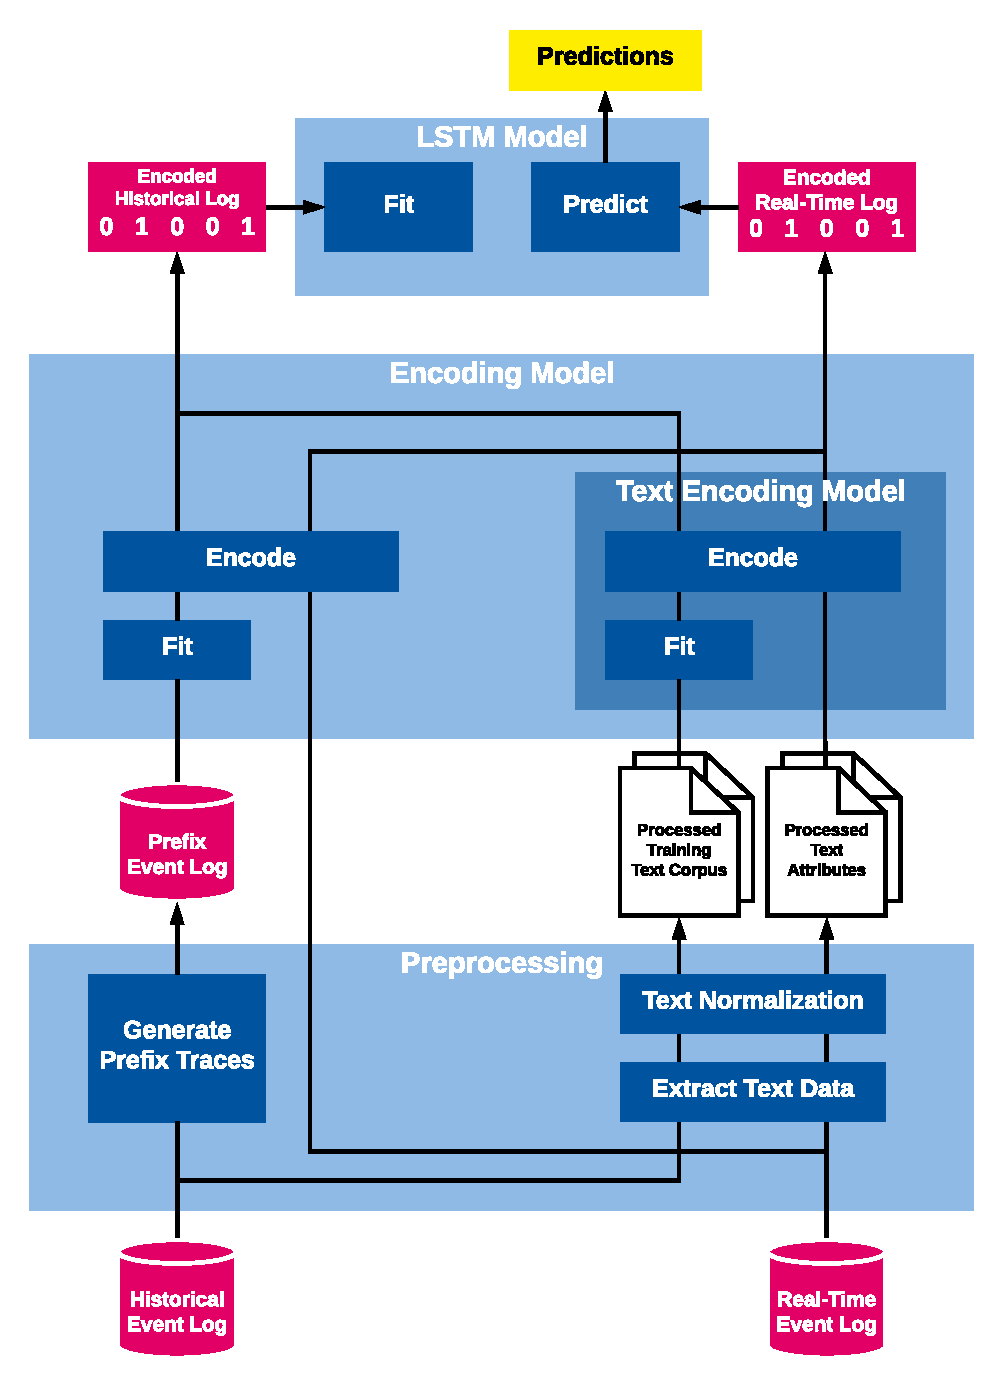
\includegraphics[width=\textwidth]{figures/framework}
	\caption[Overview of the text-aware process prediction framework]{Overview of the text-aware process prediction framework.}
	\label{fig:framework}
\end{figure}

Each encoded prefix sequence with its desired prediction target values corresponds to one training example for an LSTM network, that realizes the predictions. 
The target values of a prefix sequence are the activity and timestamp (relative to the case start) of the next event as well as the case outcome and case cycle time.
The case outcome can be for example a binary label, ie. a label telling if the case is successful or has failed or if it has been approved or declined.
In some applications the case outcome is defined by the final event of a case.
For completed cases the next activity is an artificial "PROCESS END" activity with the same timestamp as the final event.
The total number of training examples that can be generated out of the log is $\sum_{\sigma \in \eventlog}|\sigma|$, which is exactly the number of events in the log.
In the online phase, the model can be used to predict the next event, outcome and cycle time of new unseen and unfinished cases, that are currently monitored.


\section{Event Encoding}\label{sec:event}

In the offline training phase as well as during online prediction, traces are encoded as sequences of event vectors.
The prefix log $\eventlog_\mathrm{prefix}$ is encoded as training set in the offline phase, while in the online phase, running cases are encoded for prediction.
Strictly speaking, a set of encoding functions  $enc_k \colon \mathcal{E}^k \to (\mathbb{R}^n)^k$ is realized by the encoding component, that encodes (prefix-)traces of length $k$ to vector sequences of the same size, i.e. $enc_k(\sigma) = \langle \vec{x_1}, \vec{x_2}, \dots, \vec{x_k}\rangle$ with $\sigma = \langle e_1, e_2, \dots, e_k\rangle$.
Each event $e_i$ is encoded as a fixed-length vector using the activity, timestamp and additional categorical, numerical and textual data, that is associated with each event.
We assume to have $r \in \mathbb{N}_0$ numerical, $s \in \mathbb{N}_0$ categorical and $u \in \mathbb{N}_0$ textual attributes, i.e. $e_i \in \mathcal{C} \times \mathcal{A}  \times \mathcal{T} \times \mathcal{D}_1^\mathrm{num} \times \dots \times \mathcal{D}_r^\mathrm{num}   \times \mathcal{D}_1^\mathrm{cat}  \times  \dots  \times \mathcal{D}_s^\mathrm{cat}   \times \mathcal{D}_1^\mathrm{text}   \times \dots  \times \mathcal{D}_u^\mathrm{text}$.
Each encoded event vector $\vec{x_i}$ is the concatenation of set of feature vectors, which are constructed from the event data.
\begin{equation*}
\vec{x_i}=(
\vec{a_i},
\vec{t_i},
\vec{d}_{i1}^\mathrm{num}, \dots,\vec{d}_{ir}^\mathrm{num},
\vec{d}_{i1}^\mathrm{cat}, \dots,\vec{d}_{is}^\mathrm{cat},
\vec{d}_{i1}^\mathrm{text}, \dots, \vec{d}_{iu}^\mathrm{text})
\end{equation*}
The activity of the event is represented by vector $\vec{a_i}$ using \textit{one-hot encoding}.
Given the set of possible activities $\mathcal{A}$, an arbitrary but fixed ordering over is introduced with a bijective index function $index_\mathcal{A} \colon \mathcal{A} \to \{1, \dots, |\mathcal{A}|\}$.
Using this function, the activity is encoded as a vector of size $|\mathcal{A}|$, where the component $index_\mathcal{A}(\pi_\mathcal{A}(e))$ has value 1 and all the other components have value 0.
We write $\mathds{1}_\mathcal{A}\colon \mathcal{A} \to \{0,1\}^\mathcal{A}$ to describe the function that realizes such an one-hot encoding transformation for the set of all activities $\mathcal{A}$.
The timestamp of the event is used to compute a vector $\vec{t_i}$ of time-related features, which is explained in detail in Section \ref*{sec:time}.

\begin{table}[!htbp]
	\renewcommand{\arraystretch}{1.2}
	\setlength\tabcolsep{5pt}
	\begin{tabularx}{\textwidth}{p{2cm} l l p{6.8cm} }
		\toprule
		\textbf{Feature} \newline \textbf{Vector} & \textbf{Construction} &\textbf{Dimension} &  \textbf{Description} \\
		\midrule
		$\vec{a_i}$ &$\mathds{1}_\mathcal{A}(\pi_\mathcal{A}(e_i))$& $|\mathcal{A}|$& One-hot encoding of the activity. \\
		$\vec{t_i}$ & See Section \ref{sec:time} &6 & Time-based feature vector.\\
		$\vec{d}_i^\mathrm{num}$ &  $norm(\pi_{\mathcal{D}_j^\mathrm{num}}(e_i)) $ &1 & Normalized value of the $j$-th numerical attribute\\
		$\vec{d}_i^\mathrm{cat}$ & $\mathds{1}(\pi_{\mathcal{D}_j^\mathrm{cat}}(e_i))$&$|\mathcal{D}_j^\mathrm{cat}|$ & One-hot encoding of the $j$-th categorical attribute.\\
		$\vec{d}_i^\mathrm{text}$ & See Section \ref{sec:text} & $z_i$& Fixed-length vectorization of the $j$-th text attribute.\\
		\bottomrule
	\end{tabularx}
	\caption[Feature vectors as part of the event encoding]{Feature vectors as part of the event encoding $\vec{x_i}$.}
	\label{tab:features}
\end{table}

Additional attributes of the events are encoded based on their type, i.e. if they are numerical, categorical or textual.
All additional numerical attributes $\pi_{\mathcal{D}_i^\mathrm{num}} (e_i)$ are scaled to the interval $ [0, 1]$ to improve learning efficiency using min-max normalizing.
The scaling for a numerical feature $x$ is realized with the transformation

$$\hat{x} = \dfrac{x-\min(x)}{\max(x) - \min(x)},$$

where $\min(x)$ is the lowest and $\max(x)$ is the highest value $x$ can take.
If the limits are not bounded conceptually, the lowest or highest value of $x$ in the event log is used for scaling.

Categorical attributes are encoded using one-hot-encoding in the same way as the activity, i.e. $d_{ij} = \mathds{1}_{\mathcal{D}_j^{\mathrm{cat}}}$.
Textual attributes are vectorized via a dedicated text model, that is explained in Section \ref{sec:text}.

All in all, the encoding results in vector of size
\begin{equation*}
|\vec{x_i}|= |\mathcal{A}| + r + \sum_{i=1}^{s} |\mathcal{D}_i| + \sum_{j=1}^{u} z_j + 6.
\end{equation*}


\section{Capturing Temporal Dependencies}\label{sec:time}

A set of time-based features is computed from the timestamp data in the event log in order to profit from time-related pattern in the process.
As part of the complete encoding $\vec{x}_i$ for an event $e_i$ in a (prefix-)trace $\sigma = \langle e_1, \dots, e_k \rangle$ a time vector $\vec{t_i} = (t_i^1, t_i^2,t_i^3,t_i^4,t_i^5,t_i^6)$ of dimension 6 is computed.

\begin{table}[!htbp]
	\centering
	\begin{tabularx}{0.6\textwidth}{l l}
		\toprule
		 \textbf{Feature} & \textbf{Description} \\
		 \midrule
		$t_i^1$ & Time since previous event \\
		$t_i^2$ & Time since case start \\
		$t_i^3$ & Time since first recorded event \\
		$t_i^4$ & Time since midnight \\
		$t_i^5$ & Time since last Monday \\
		$t_i^6$ & Time since last January 1 00:00 \\
		\bottomrule
	\end{tabularx}
	\caption[Time-based features as part of the event encoding]{Time-based features as part of event encoding $\vec{x_i}$.}
	\label{tab:time-features}
\end{table}

Using the time features a set of time-dependent trends can be captured and utilized for prediction.
The feature $t_i^1$ describes the time difference between the current event $e_i$ and previous event $e_{i-1}$, while $t_i^2$ gives the time difference between the current event and the first event of the case $e_1$, i.e. the time since the start of the case.
Furthermore, $t_i^3$ is the time difference between the current event and the first event that is recorded in the log. This feature indicates the absolute time position of an event in the data.
This information is important to detect concept drift in the process \cite{DBLP:journals/tnn/BoseAZP14}.
Most real-life processes are not static, i.e. the behavior of the process changes over time.
For example, in earlier process executions customers might have been informed by a letter, whereas in more recent cases customers are messaged using email or app notifications.
Therefore, the knowledge about the absolute time of the events can be used to relate cases in similar periods of time.

The features $t_i^4, t_i^5$ and $t_i^6$ capture the time difference between the current event and midnight, the current event and the most recent monday and the current event and the beginning of the year. They are used to capture daily, weekly and seasonal trends.
For example, some activities might only be executed during office hours or before the weekend.
Also, many businesses expect seasonally fluctuating demand, for example a booking platform usually has much more customers in summer, which can affect the process execution in many ways.
Each feature $t_i^1, \dots, t_i^6$ is min-max normalized such that $t_i^j \in [0,1]$ for $j \in [6]$.
A summary of all time-related features can be seen in Table \ref{tab:time-features}.

\section{Text Vectorization}\label{sec:text}

In order to prepare the textual data of the event log for a prediction model, the texts have to be encoded in a compact, finite and "useful" numerical vector representationu using a text model.
Useful in that context means, that texts with similar semantic meanings should also have similar representations.
The vector representation of text data is an important aspect in \textit{Natural Language Processing} (NLP).
Extracting the meaning of textual information remains a challenge even for humans, because textual data is unstructured, language dependent and domain specific.
Many words are ambiguous, for example the word "apple" might denote a fruit or a global technology company.
In addition, grammatical variations and the importance of context in language makes extracting the semantic meaning even more difficult for computers.

In our setting, the text vectorization for textual attributes is realized in a two step procedure by text encoding component.
First, all text data associated with the events in the corresponding textual attribute is collected in a so called \textit{text corpus}.
Each document in the text corpus is then preprocessed in order to filter out linguistic noise or useless information.
This step is called \textit{text normalization}.
Finally, the normalized text corpus is used to build up a \textit{vocabulary} and a text vectorization technique is applied to encode the text of the attribute into a fixed-length vector.
The vocabulary of a text corpus is a set $V$ of all relevant words that appear in the corpus and is indexed by an bijective index function $index_V \colon V \to \{1, 2, \dots, |V|\}$.
As text vectorization techniques rely on the Bag of Words, Bag of N-Grams, Paragraph Vector or Latent Dirichlet Allocation as a text model.

\subsection{Text Normalization}

In the text normalization step each document of the text corpus is transformed by a preprocessing pipeline which consists of the following four steps:

\begin{enumerate} 
	\item Letters are converted to lowercase
	\item Document is tokenized (i.e. splitted) by word
	\item Each word is lemmatized
	\item Stop words are filtered out
\end{enumerate}

The first step eliminates all capital letters in the text.
In the tokenenization step a document is split up in a sequence of words.
Each word is then lemmatized, i.e. it is converted to its canonical form.
The idea is to unify words that have a very similar meaning and filter out grammatical variations.
For example, the words  "go", "going", "goes", "gone" and "went" are all transformed to the basic form "go".

Ultimately, all stop words are filtered out of each document.
Stop words are words with low information value like "the", "a", "of" or "here".
Stop word lists are language dependent and can be more or less aggressive at filtering.
Usually they contains articles, auxiliary verbs, prepositions and generic verbs like "be" and "have".
In addition, punctuation marks and numerical information are excluded.

\begin{table}[!htbp]
	\begin{tabularx}{\textwidth}{l l p{9.8cm}}
		\toprule
		\textbf{Step} & \textbf{Transformation} & \textbf{Example Document}                                                       \\ \midrule
		0             & Original       & "The patient has been diagnosed with high blood pressure." \\
		1             & Lowercase               & "the patient has been diagnosed with high blood pressure." \\
		2 & Tokenization  & $\langle$"the", "patient", "has", "been", "diagnosed", "with", "high", "blood", "pressure", "."$\rangle$ \\
		3 & Lemmatization & $\langle$"the", "patient", "have", "be", "diagnose", "with", "high", "blood", "pressure", "."$\rangle$  \\
		4             & Stop word filtering     & $\langle$"patient", "diagnose", "high", "blood", "pressure"$\rangle$ \\ \bottomrule
	\end{tabularx}
	\caption[Preprocessing transformation of an example document]{Preprocessing transformation of an example document containing a single sentence.}
	\label{tab:text-preprocessing}
\end{table}


\subsection{Bag of Words}

The \textit{Bag of Words} (BoW) model is a simple text model, which represents documents based on the \textit{term frequencies} of its words, while ignoring their order \cite{harris1954distributional}.
Given the learned vocabulary $V$ a document is represented by a vector of size $|V|$, where the $i$-th component gives the number of occurrences of the word in the document indexed with $i$ it.

Since this approach does not reflect the prior distributions of words in the corpus, i.e. how likely certain words appear in a document in general, the term frequencies are usually normalized by the so-called \textit{inverse document frequency} (idf) of a word.
The inverse document frequency indicates the specificity of a word in the corpus and is computed by dividing the total number of documents by the number of documents that contain the specific word and scaling that value logarithmically.
The resulting score is the tfidf score of a word in a document.
 consul

The Bag of Words model is easy to build and effective for certain applications, but limited in several ways.
First, the model completely ignores the order of words, which is often crucial for understanding the semantic meaning. For example, the sentences "The patient's health state went from stable to critical." and "The patient's health state went from critical to stable." would result in the same vector representation, while the meaning is clearly inverted.
Second, the vector representations are sparse and of high dimensionality since they depend of the size of the vocabulary.
However, the dimension can be reduced by limiting the size of the vocabulary. For example, words with low tfidf scores can excluded from the vocabulary.


\subsection{Bag of N-Grams}

The \textit{Bag of N-Grams} model is a generalization of the Bag-of-Words model, which addresses the missing word order awareness of the latter.
Instead of single words, the vocabulary consists of $n$-tuples of words, that appear consecutive in the corpus.
The unigram model ($n=1$) is equivalent to the BoW model.
For the bigram model ($n=2$), the vocabulary consists of pairs of words that appear next to each other in the documents.
For example, for the preprocessed document $\langle$"patient", "diagnose", "high", "blood", "pressure"$\rangle$, the pairs ("patient", "diagnose"), ("diagnose", "high"), ("high", "blood") and ("blood", "pressure") are taken into the vocabulary.
For $n>2$ n-tuples are generated accordingly.
The feature vector is constructed by computing the tfidf score for each vocabulary entry like in the BoW model.

Compared to the BoW model, n-grams also take the order of words into account, which is beneficent in many scenarios.
However, the vocabulary size is usually even higher than in the BoW model.
In order to generate more compact vectors, distributed text representations are needed for larger text corpora and vocabularies.



\subsection{Paragraph Vector}

The \textit{Paragraph Vector} also known as \textit{Doc2Vec}, originally presented by \citeauthor{DBLP:conf/icml/LeM14} in \citeyear{DBLP:conf/icml/LeM14}, is an unsupervised algorithm that learns distributed fixed length vector representations for documents of variable length \cite{DBLP:conf/icml/LeM14}.
The idea is inspired by the word embedding model presented by \citeauthor{DBLP:journals/jmlr/BengioDVJ03} \cite{DBLP:journals/jmlr/BengioDVJ03}, which can learn distributed fixed-length vector representations for words.
In this model words are mapped to vectors, that are trained to predict words from its context, i.e. words that appear before or after the target word in the training documents.
Several variants of this approach exits, notably the \textit{Continuous Bag of Words} model, which ignores the order of the words in the context and the \textit{Continuous Skip-gram} model, which predicts the skip-gram context for a word vector (also known as \textit{Word2Vec})\cite{DBLP:journals/corr/abs-1301-3781}.

\begin{figure}[!htbp]
	\centering
	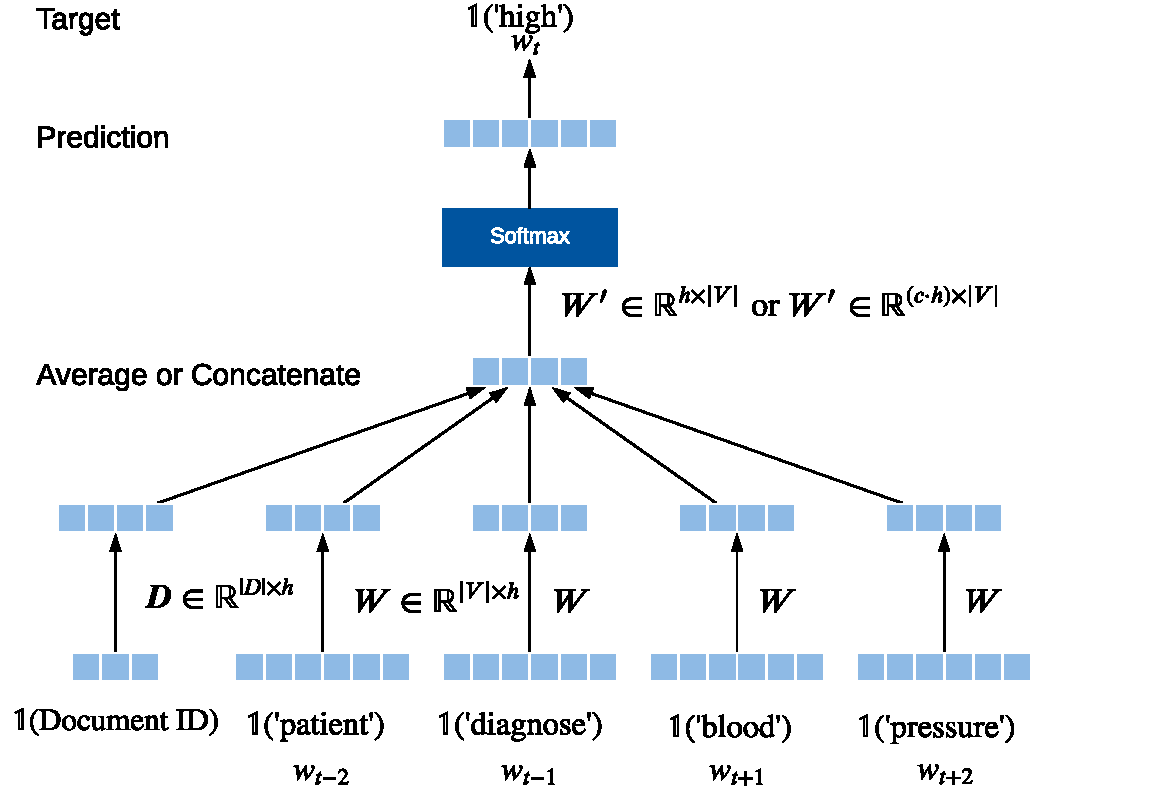
\includegraphics[width=\textwidth]{figures/paragraph-vector}
	\caption[Distributed memory paragraph vector model]{The distributed memory paragraph vector model (PV-DM) is designed to predict a word $w_t$ from its context and derives fixed-length representation of documents and words via the learned matrices $\vec{D}$ and $\vec{W}$.}
	\label{fig:paragraph-vector}
\end{figure}

The core idea of the paragraph vector model is to extend the model in \cite{DBLP:journals/jmlr/BengioDVJ03} in a way, that an additional document or paragraph vector, that is unique per document is trained together with the word vectors.
Fig. \ref{fig:paragraph-vector} show the architecture of the distributed memory variant of the paragraph vector model (PV-DM).
Its is realized by a neural network, that takes one-hot encoded words and a one-hot encoded document IDs as input.
These are mapped to vector representation via weight matrices $\vec{D}$ and $\vec{W}$, which are learned during training with gradient descent.
The distributed representations are then averaged or concatenated to a vector in order to predict the one-hot encoded target word using another mapping via $\vec{W'}$ and a softmax activation function.
The training set is constructed using a sliding window over every document, such that the input is the context of the target word and the document ID.
After training, each column in $\vec{D}$ represents the distributed encoding of the corresponding document.

The network is also able to learn a representation for new unseen documents by an inference step.
In this phase, the word matrix $\vec{W}$ and the prediction matrix $\vec{W'}$ are fixed and only the document vector is trained.
The paragraph vector model tends to perform better than non-distributed models, however since new documents are vectorized via inference, a bigger training corpus of documents is usually required.

\subsection{Latent Dirichlet Allocation}

The Latent Dirichlet Allocation presented by \citeauthor{DBLP:journals/jmlr/BleiNJ03} in \citeyear{DBLP:journals/jmlr/BleiNJ03} \cite{DBLP:journals/jmlr/BleiNJ03} is generative statistical text model, that represents documents as a mixture of a fixed number of topics, depending on the words of the document.
Therefore, a document is encoded as a vector whose dimension is equal to the number of chosen topics and each component indicates the degree of affiliation between the document and the corresponding topic.
The topics are are not generated manually, but by the model itself.

\section{Network Architecture and Training}

The LSTM network is designed to be trained with all prediction targets (next activity, next event time, case outcome and case cycle time) at once, in order to benefit from correlations between these.
The network consists of an input layer, an shared LSTM layer, an a specialized LSTM layer for each target, and an fully connected output layer for each target.
Furthermore, layer normalization \cite{DBLP:journals/corr/BaKH16} is applied after each LSTM layer, which standardizes the hidden output in order to speed up the training convergence.

\begin{figure}[!htbp]
	\centering
	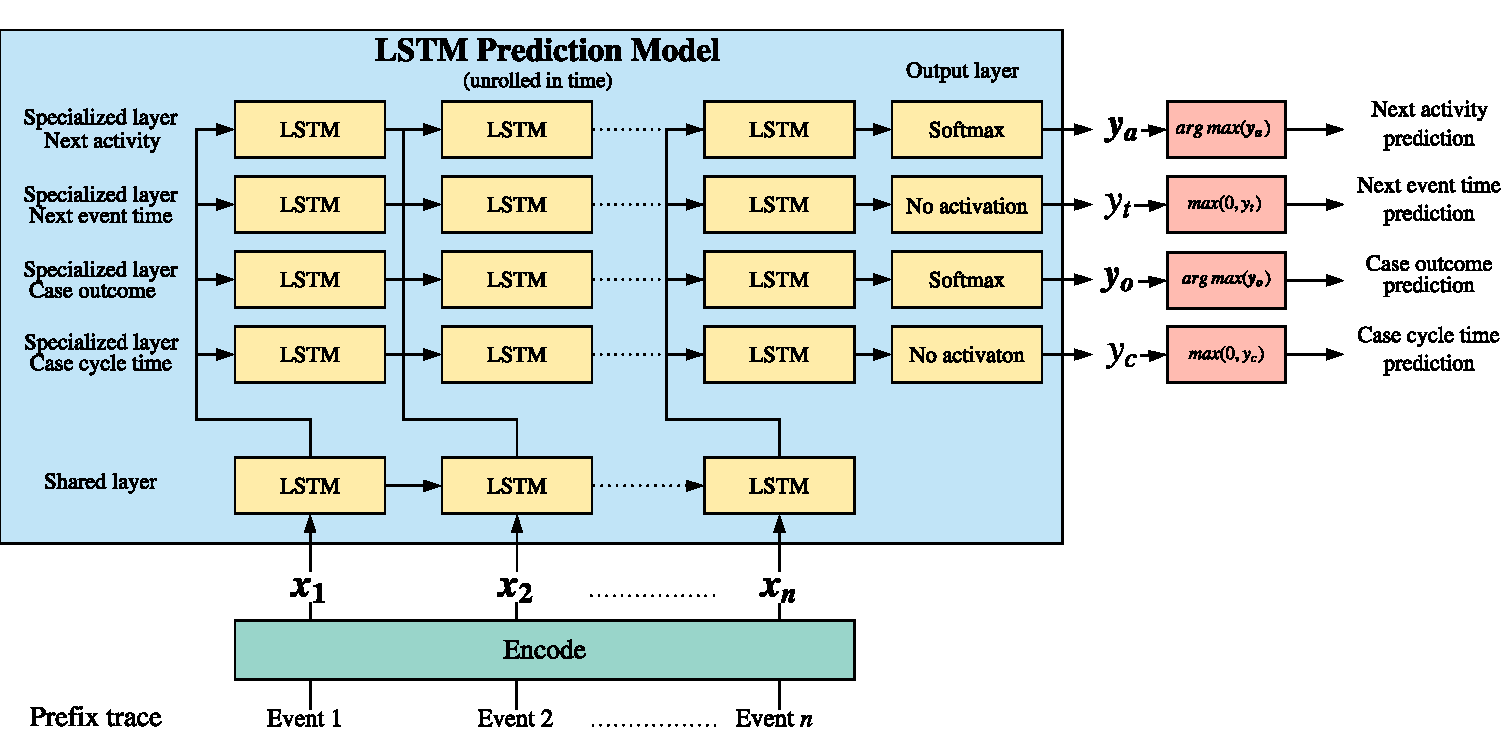
\includegraphics[width=\textwidth]{figures/network}
	\caption[LSTM model for text-aware process prediction]{LSTM model to simultaneously predict the next activity $(\vec{y_a})$, next event time$(y_t)$, case outcome $(\vec{y_o})$ and case cylce time $(y_c)$ for an encoded prefix trace $\vec{x_1}, \vec{x_2}, \dots, \vec{x_n}$.}
	\label{fig:network}
\end{figure}

The fully connected output layer uses a softmax activation function for the next activity and case outcome prediction to estimate the probability for each target value.
The function normalizes a vector of real numbers into another vector of same dimension such that all component are in the interval (0,1) and the sum of all component is equal to 1.
Hence, the transformed vector can be interpreted as a probability distribution, while keeping the proportions of the original vector.
The softmax function is described with
\begin{equation*}\label{key}
	\text{Softmax}(\vec{x})_i = \frac{\exp(x_i)}{\sum_{j=1}^{n} \exp(x_j)}  \; \text{for} \, i = 1, \dots, n \text{ and } \vec{x}=(x_1, \dots, x_n) \in \mathbb{R}^n.
\end{equation*}
The training set of encoded prefix traces is represented by an 3-dimensional matrix of real values, where the three dimensions specify the prefix traces, the events per prefix trace and the features per event.
Since the prefix traces have different length, shorter traces are pre-padded \cite{DBLP:journals/corr/abs-1903-07288} with zeros vectors.
Hence, a prefix trace of encoded events $\vec{x_1}, \vec{x_2}, \dots, \vec{x_n}$  is represented in the training set by a 2-dimensional matrix $(\mathbf{0}, \dots, \mathbf{0},\vec{x_1}, \vec{x_2}, \dots, \vec{x_n})$, such that the zero vectors fill up shorter traces to the length of the longest trace in the training set.
All prefix traces together form the 3-dimensional training matrix.

The training is realized by a backpropagation through time (BPTT) algorithm that updates the weights of the network using the update rules of the Adam optimizer with Nesterov momentum \cite{dozat2016incorporating}.
The loss for numerical prediction values $\hat{y}$ and the true value $y$ is the absolute error $\text{AE}(\hat{y},y)=|\hat{y} - y|$, while the loss for categorical prediction values is computed using the categorical cross entropy error $\text{CE} = - \sum_{i=1}^{k} y_i \cdot \log \hat{y}_i$.


\section{Predictive Business Processing Monitoring}

During online business process monitoring, predictions are realized by a forward-pass of the encoded running cases through the LSTM model.
The component with the highest value of the softmax outputs for the next activity $(\vec{y_a})$ and the case outcome $(\vec{y_o})$ indicates the categorical prediction.
The output values for the next event time $(y_t)$ and case duration  $(y_c)$ are clipped to 0 for negative outputs and the normalization is reverted, in order to compute the final prediction value.
